\documentclass[10pt]{scrartcl}
\usepackage{fullpage}
\usepackage{comment}
\usepackage{amsmath,amsfonts,amsthm,bm}
\usepackage{mathtools}
\usepackage{amsthm}
\usepackage{enumerate}
\usepackage{algpseudocode} 
\usepackage{graphicx}
\usepackage{float}
\usepackage{hyperref}
%\usepackage{subfigure}
\usepackage{caption}
\usepackage{subcaption}
\usepackage{amssymb}

\setlength{\parskip}{1em}  % Increase paragraph spacing.
\setlength\parindent{0pt}   % No indentation before paragraph.


%%%% Macros
\newcommand{\R}{\mathbb{R}}                       % Reals.
\newcommand{\vx}{\mathbf{x}}                        % vector x..
\newcommand{\dX}{\mathcal{X}}                     % Domain X.
\newcommand{\valpha}{\boldsymbol{\alpha}}  % vector alpha.


\title{CS57800: Preliminary Project Report}
\author{Shraddha Parimita Sahoo \& Vinoth Venkatesan \\ (sahoo0, venkat26)@purdue.edu} % Put your name and Purdue email on this line

\begin{comment}
I expect around 30-40\% of what will be in your final report.

Therefore, at this point source code should include ALL the data preprocessing (e.g., reading the original format of the data, computing features, putting the data in table format, etc.), running SOME of the algorithms in your plan, and PART of the implementation of cross-validation. (Code for generating figures and tables of the experimental results such as charts, ROC curves, etc. are not required yet.)

//Write about the data features and the target output (0-9 digits)
//Write about all the algorithms, what they achieve, their formula (for SVM, KNN, Neural Net)
\end{comment}

\date{}

\begin{document}
%\pagenumbering{gobble}
\maketitle
\section*{Introduction} 
The aim of the project is to study the performance of various classification algorithms, namely, Support Vector Machines (SVM), K-nearest neighbors (KNN), and neutral networks. We evaluate these algorithms on the task of identifying handwritten digits.  The details of the data set and the pre-processing that was done
is described next.

\subsection*{Data set Preprocessing}
The MNIST data set, which is a subset of a bigger data set from National Institute of Standards and Technology (NIST),
is a collection of handwritten digits, each between 0 to 9, and is commonly used as a benchmark data set for evaluating various image processing systems.
The data set has a training set of 60,000 examples, and a test set of 10,000 examples.

The original NIST data set which was black and white (i.e. had only two levels) was first processed to fit into a $20 \times 20$ pixel image. 
Each image was then smoothed (anti-aliased) to obtain a grey-scale image which was then centered in a $28 \times 28$ pixel box.
The centering was performed by computing the center of mass of the pixels, and translating the image so as to position that point at the center of the $28 \times 28$ field. 
The data set was downloaded using the \emph{scikit-learn} python library (\texttt{fetch\_mldata} method in package \texttt{sklearn.datasets}).

Next, we describe the classification algorithms that were used in this project.

\section*{Classification Algorithms}
In this section, we describe three methods, namely, SVM, KNN and Neural network, for the task of recognizing handwritten digits. The classification
task is to learn a function that maps images of handwritten digits $\mathcal{X}$ to digits $\mathcal{Y} = \{0, 1, \ldots 9\}$,
from a data set of labeled examples (images of handwritten digits).
In our case, $\mathcal{X} = [0, 255]^{784}$ corresponds to the set of flattened $28 \times 28$ grey-scale images. 
Let $d$ ($784$ in this case) denote the dimension of the feature space and $k$ ($10$ in this case) denote the number of classes.
We have a data set $S = \{ (\vx_i, y_i)  \}_{i=1}^n$ of $n$ labeled images. 

\subsection*{Support Vector Machines}
Support Vector Machines (SVM) is one of the most widely used classification algorithm for both binary and multi-task problems.
SVM is a maximum margin classifier. To solve the multi-class problem of classifying handwritten digits, we use the all-pairs strategy
of learning ${k \choose 2}$ binary classifiers. We train each binary classifier using by solving the following optimization problem:
\begin{align*}
\hat{\valpha} = 
& \min_{\valpha \in \R^d}  \quad \sum_{i=1}^{n} \alpha_i - \frac{1}{2} \sum_{i,j=1}^{n} \alpha_i \alpha_j y_i y_j K(\vx_i,\vx_j) \\ 
& \text{ subject to } \quad  0 \leq \alpha_i \leq C, i=1,\ldots,n, \;  \sum_{i=1}^{n} \alpha_i y_i = 0,
\end{align*}
where $\alpha_i$ and $\alpha_j$ are non-negative Lagrange multipliers  used to enforce the classification constraints, 
$y_i$ and$y_j$ are predicted labels for data points $\vx_i$  and $\vx_j$ and $K$ is the kernel function.  

The prediction $y$ for a test data point $\vx \in \dX$, for each binary classifier, is then obtained as follows:
\begin{align*}
y = \mathrm{sign} \left( \sum_{i=1}^n \hat{\alpha}_i y_i K(\vx, \vx_i) \right)
\end{align*}
Finally, the class which received the most votes is selected as the predicted label. We have evaluated the performance of the \textbf{linear kernel}
in our experiments. We used \texttt{scikit-learn} python package for an implementation of the above.

\subsection*{K-Nearest Neighbors}
K-nearest neighbors (KNN) is a popular non-parameteric classification algorithm which predicts the label of data point
by computing the majority label over $K$ nearest neighbors to the data point. In the training phase, 
a data structure (KD Tree) is constructed over all training data points for efficiently performing nearest neighbor queries during prediction.
During prediction, the constructed tree is queried to find the $K$ nearest neighbors, in Euclidean distance,
 and then the majority label is predicted as the class label of the test data point. We use uniform weighting for computing the votes.

\subsection*{Neural networks}
Neural Network / Multi-Layer Perceptron (MLP) is a supervised learning algorithm that uses multiple layers of neurons (perceptrons) to learn a non-linear function $f(\cdot):\mathbb{R}^{d} \rightarrow \mathbb{R}^{k}$. It differs from logistic regression by having multiple non-linear layers between the input layer and the output layer. In our case, the input layer has a dimension of 784(d) and the output layer has a dimension of 10(k - classes). Given training data, we use backpropagation to learn the weights and biases of the perceptrons in the neural network by optimizing a cost function.

When a new test point comes in, we predict the class it belongs based on the output array (k-dimensional) from the output layer by looking at the class which has the highest vote. Various parameters like the learning rate, the activation function for the perceptrons and regularization affect the performance of the neural networks and we use a 10-fold cross-validation approach to tune these parameters. 


\section*{Experimental Set-up}
In this section we describe our experimental setup in detail.
We used 10-fold cross validation (CV) with stratified sampling to pick the optimal hyper-parameters for each algorithm, namely, 
the regularization parameter for SVM, the value of K for KNN, the best activation function, gradient descent learning rate and the regularization parameter for Neural networks. We then plot the mean cross-validation accuracy for each hyper-parameter value used for different algorithms.

After picking the best hyper-parameters for each algorithm from the above step, we ran experiments to find the effect of number of training data samples on accuracy. 
For different training data set sizes we computed the mean accuracy across $10$ randomly sampled (stratified) data sets
while keeping test samples fixed at 10,000. We then plot the test set accuracy as the number of samples is varied.

In another set of experiments, we explored the effect of using PCA (Principal Component Analysis) features on the accuracy.
We ran experiments to pick the top-K PCA features which explained 90\% of the variance in the data. We plot the variance explained
versus the number of PCA features.

We used the implementation provided by the \texttt{scikit-learn} python library for each of the above algorithms.

\paragraph{Stratified sampling}
We used stratified sampling to ensure that the relative proportion of various classes in the full data set is maintained in each of the sampled
data set. In stratified sampling the whole dataset is first partitioned into 10 groups (one group for each class 0-9). 
Then data points are sampled from each group and combined to form samples.

The experimental set-up for 10 fold cross validation, effect of varying number of training data on accuracy and PCA feature generations are explained next.
 
\section*{Experiments} 
\paragraph{10-Fold Cross Validation For Parameter Tuning.}
For 10-fold cross validation we used stratified sampling using all 70,000 MNIST data. We first divided the whole data into 10 groups (data belonging to each digit from 0-9). Then  for each fold in 10-fold CV, we picked one fold from each group and combined them to form our test data set (approximately 7,000 data points) and rest of the data i.e. the other 9-folds were our training data set (approximately 63,000 data points). The results are shown in Figure \ref{fig:svm_knn_cv} and \ref{fig:nn_cv}.

From the plots we see that, the hyper-parameter C for SVM was selected to be $\mathbf{70}$, value of K for KNN was selected to be $\mathbf{3}$ since the accuracy is highest at K=3, and in case of the neural networks, the following configuration was chosen: 

\begin{itemize}
\item Regularization parameter ($\alpha$): $100$
\item Activation function: Logistic
\item Learning rate ($\eta$): 0.0003
\end{itemize}

\begin{figure}[H]
\centering
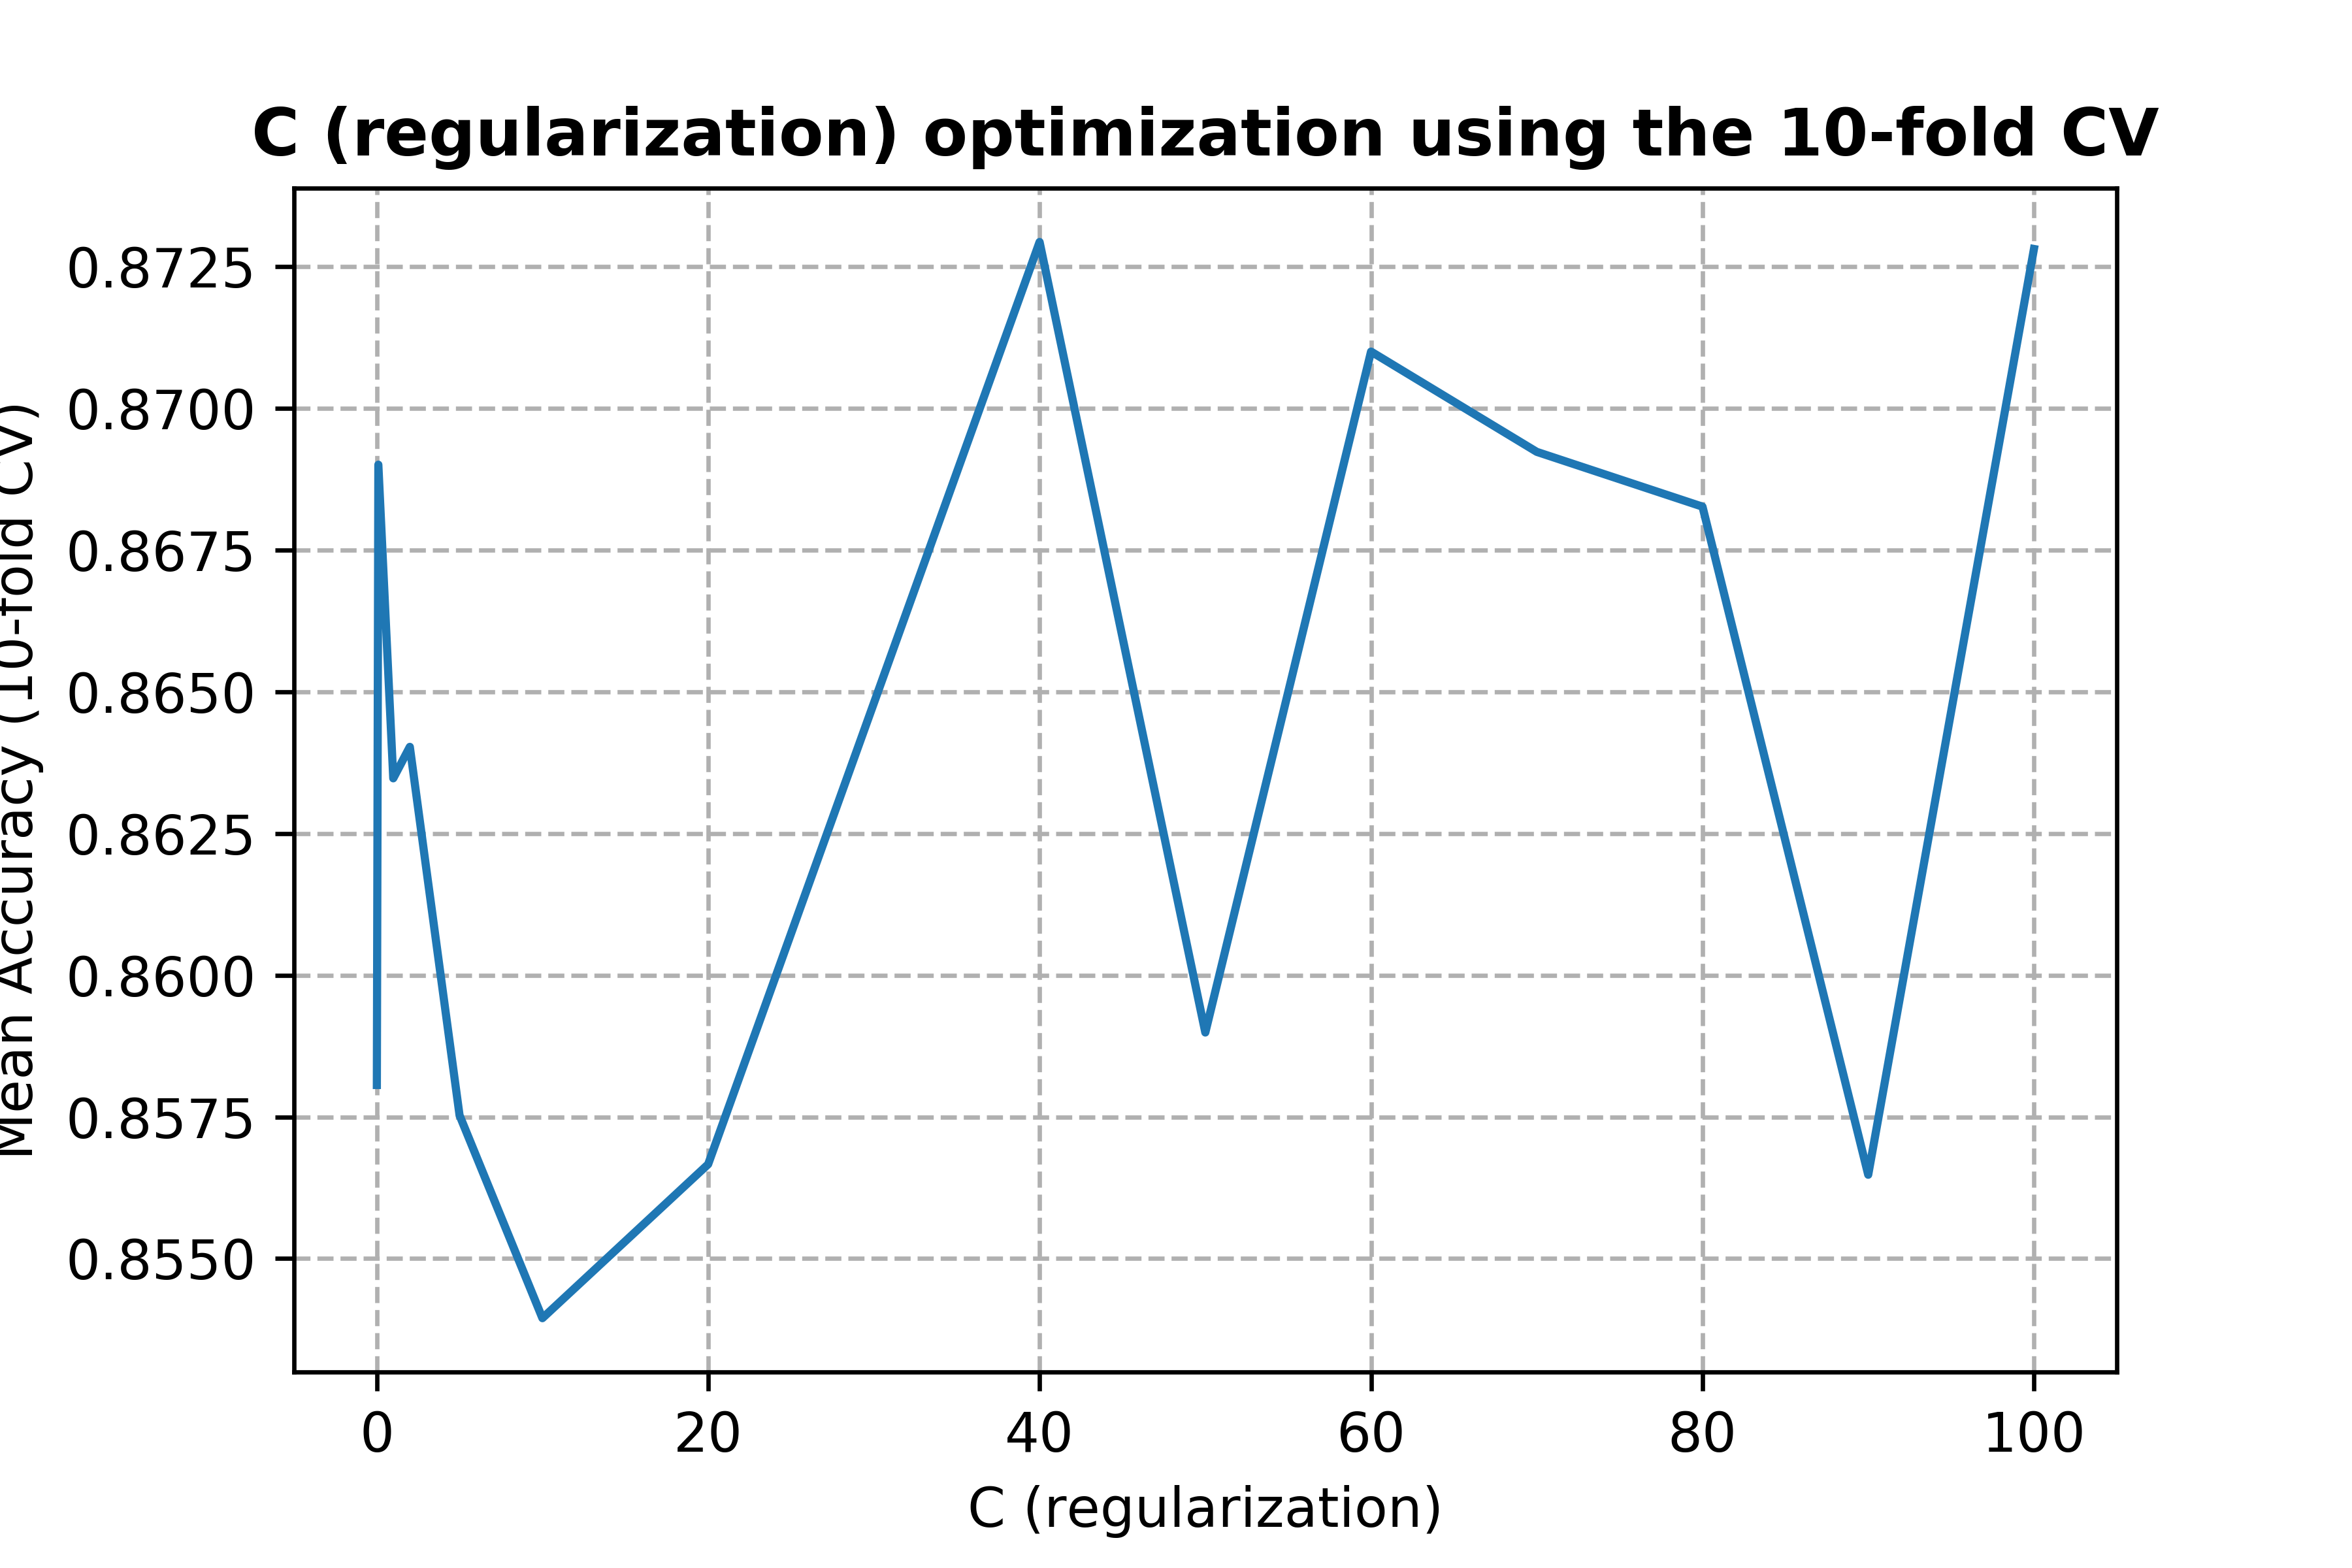
\includegraphics[width=0.45\linewidth]{figures/SVM_regularization_C_mean_acc.png}
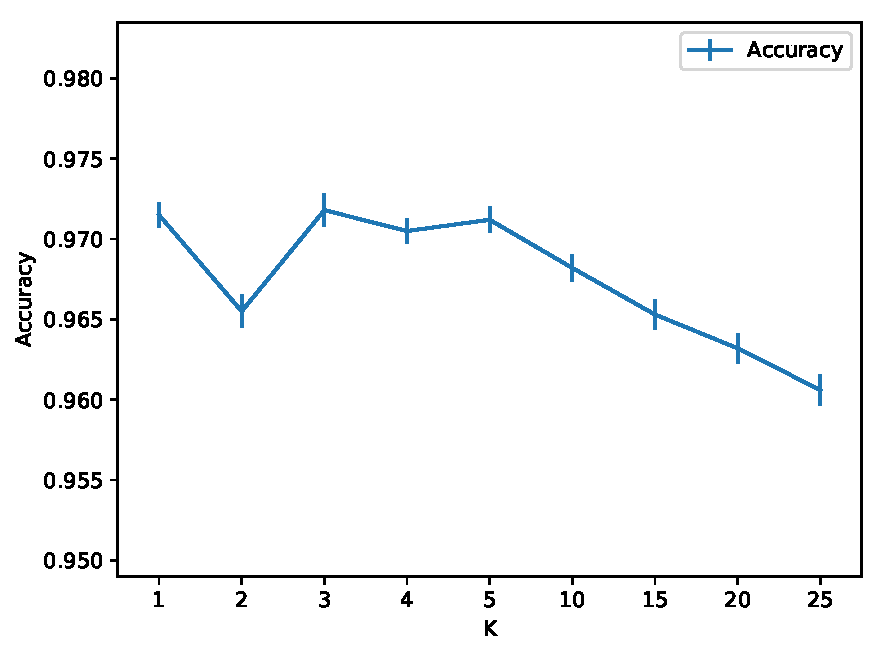
\includegraphics[width=0.4\linewidth]{figures/KNN_accuracy_vs_k_with_all_k_values.pdf}
\caption{(Left) CV for SVM. (Right) CV for KNN. \label{fig:svm_knn_cv}}
\end{figure}

\begin{figure}[H]
\centering
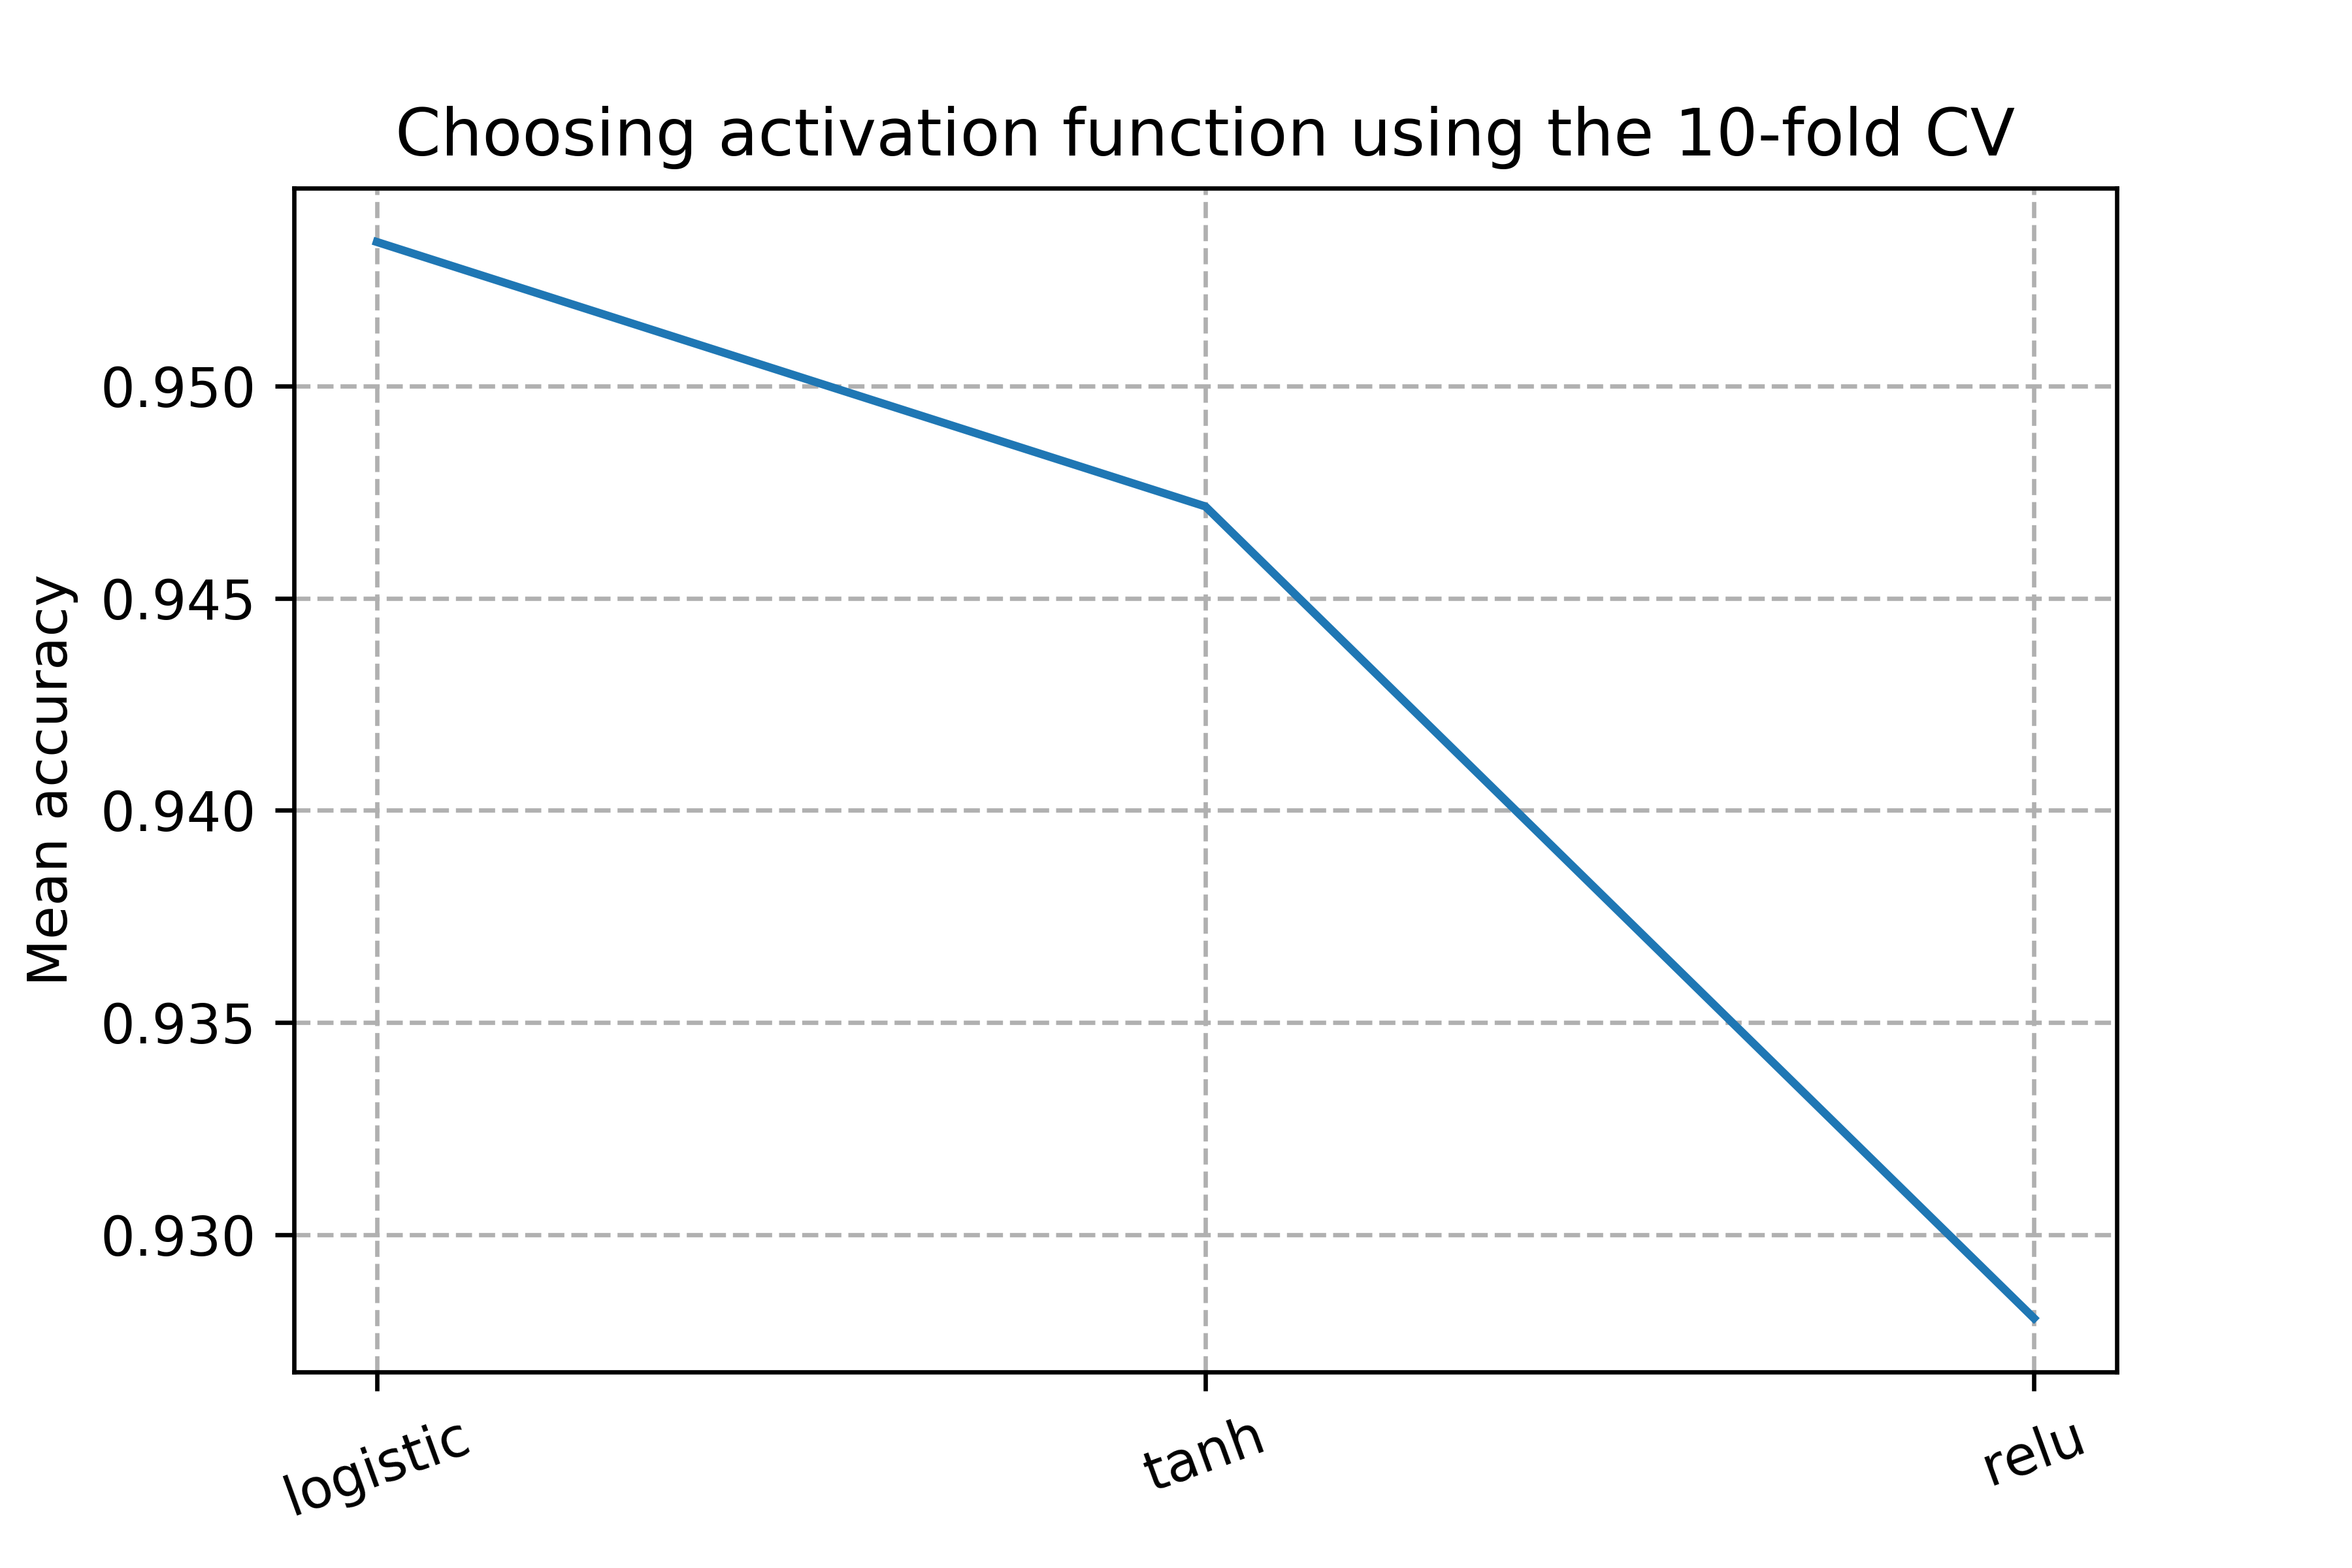
\includegraphics[width=0.33\linewidth]{figures/Neural_net_act_fcn_mean_acc.png}%
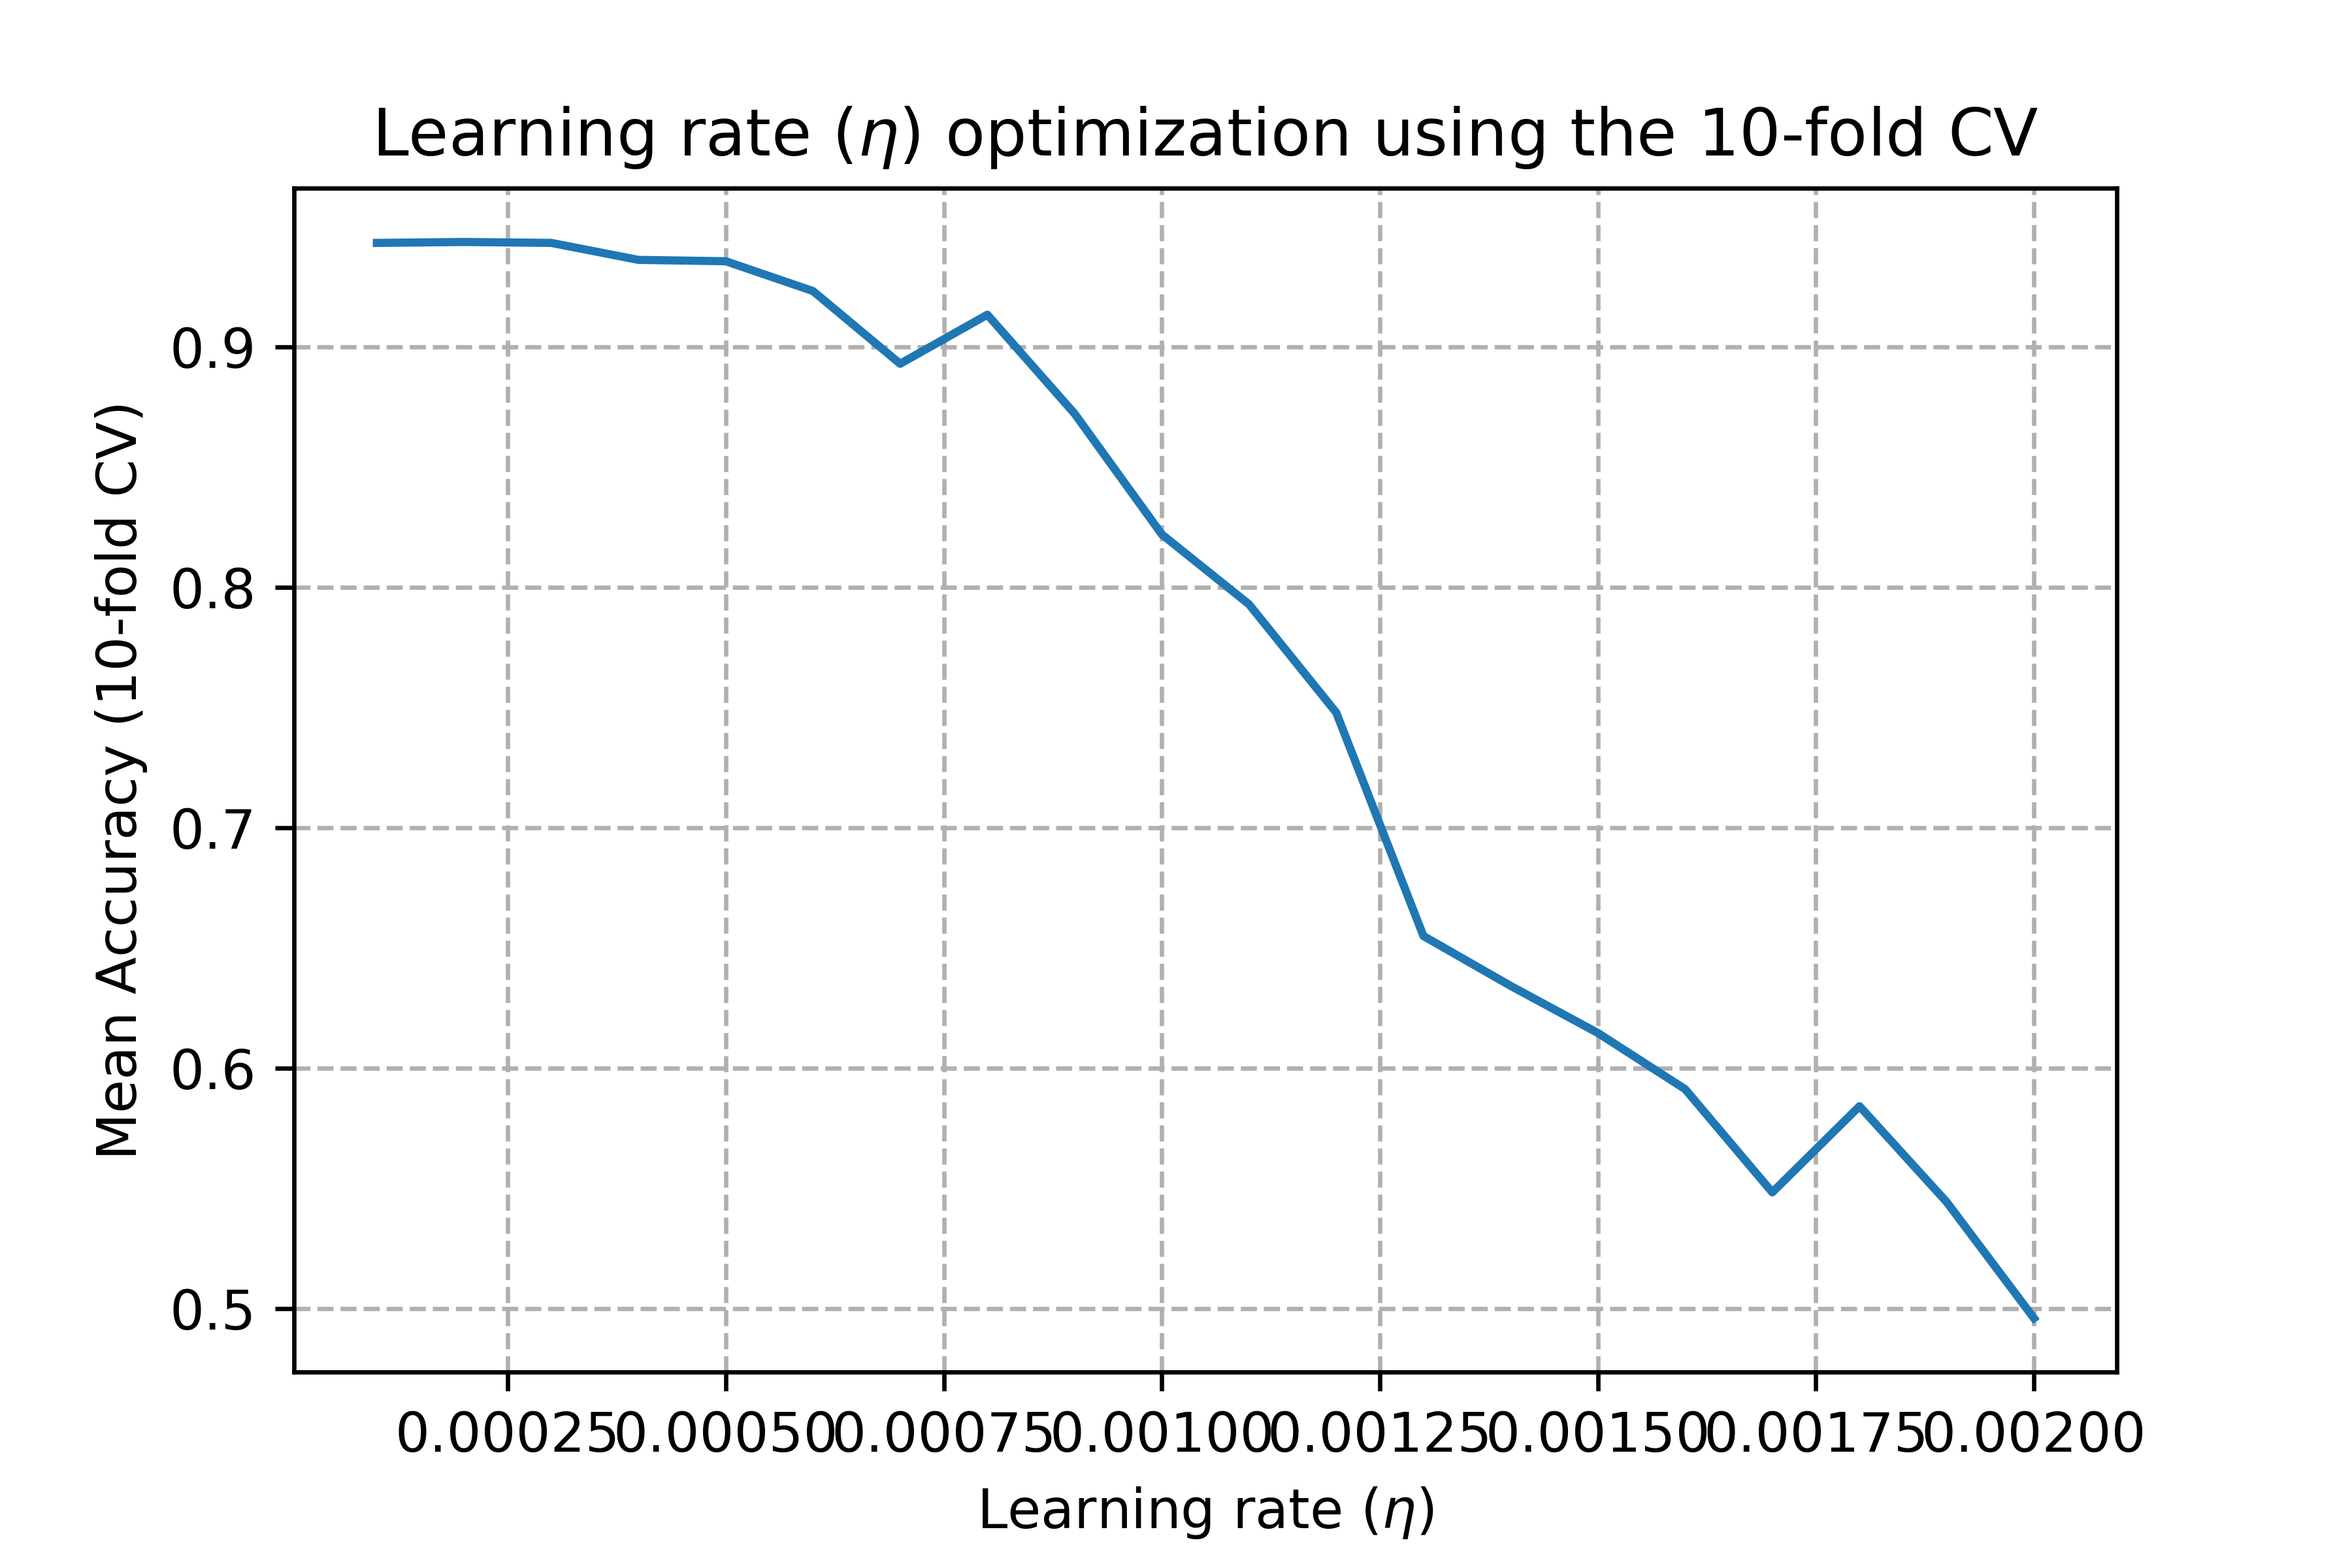
\includegraphics[width=0.33\linewidth]{figures/Neural_net_learn_rate_mean_acc.png}%
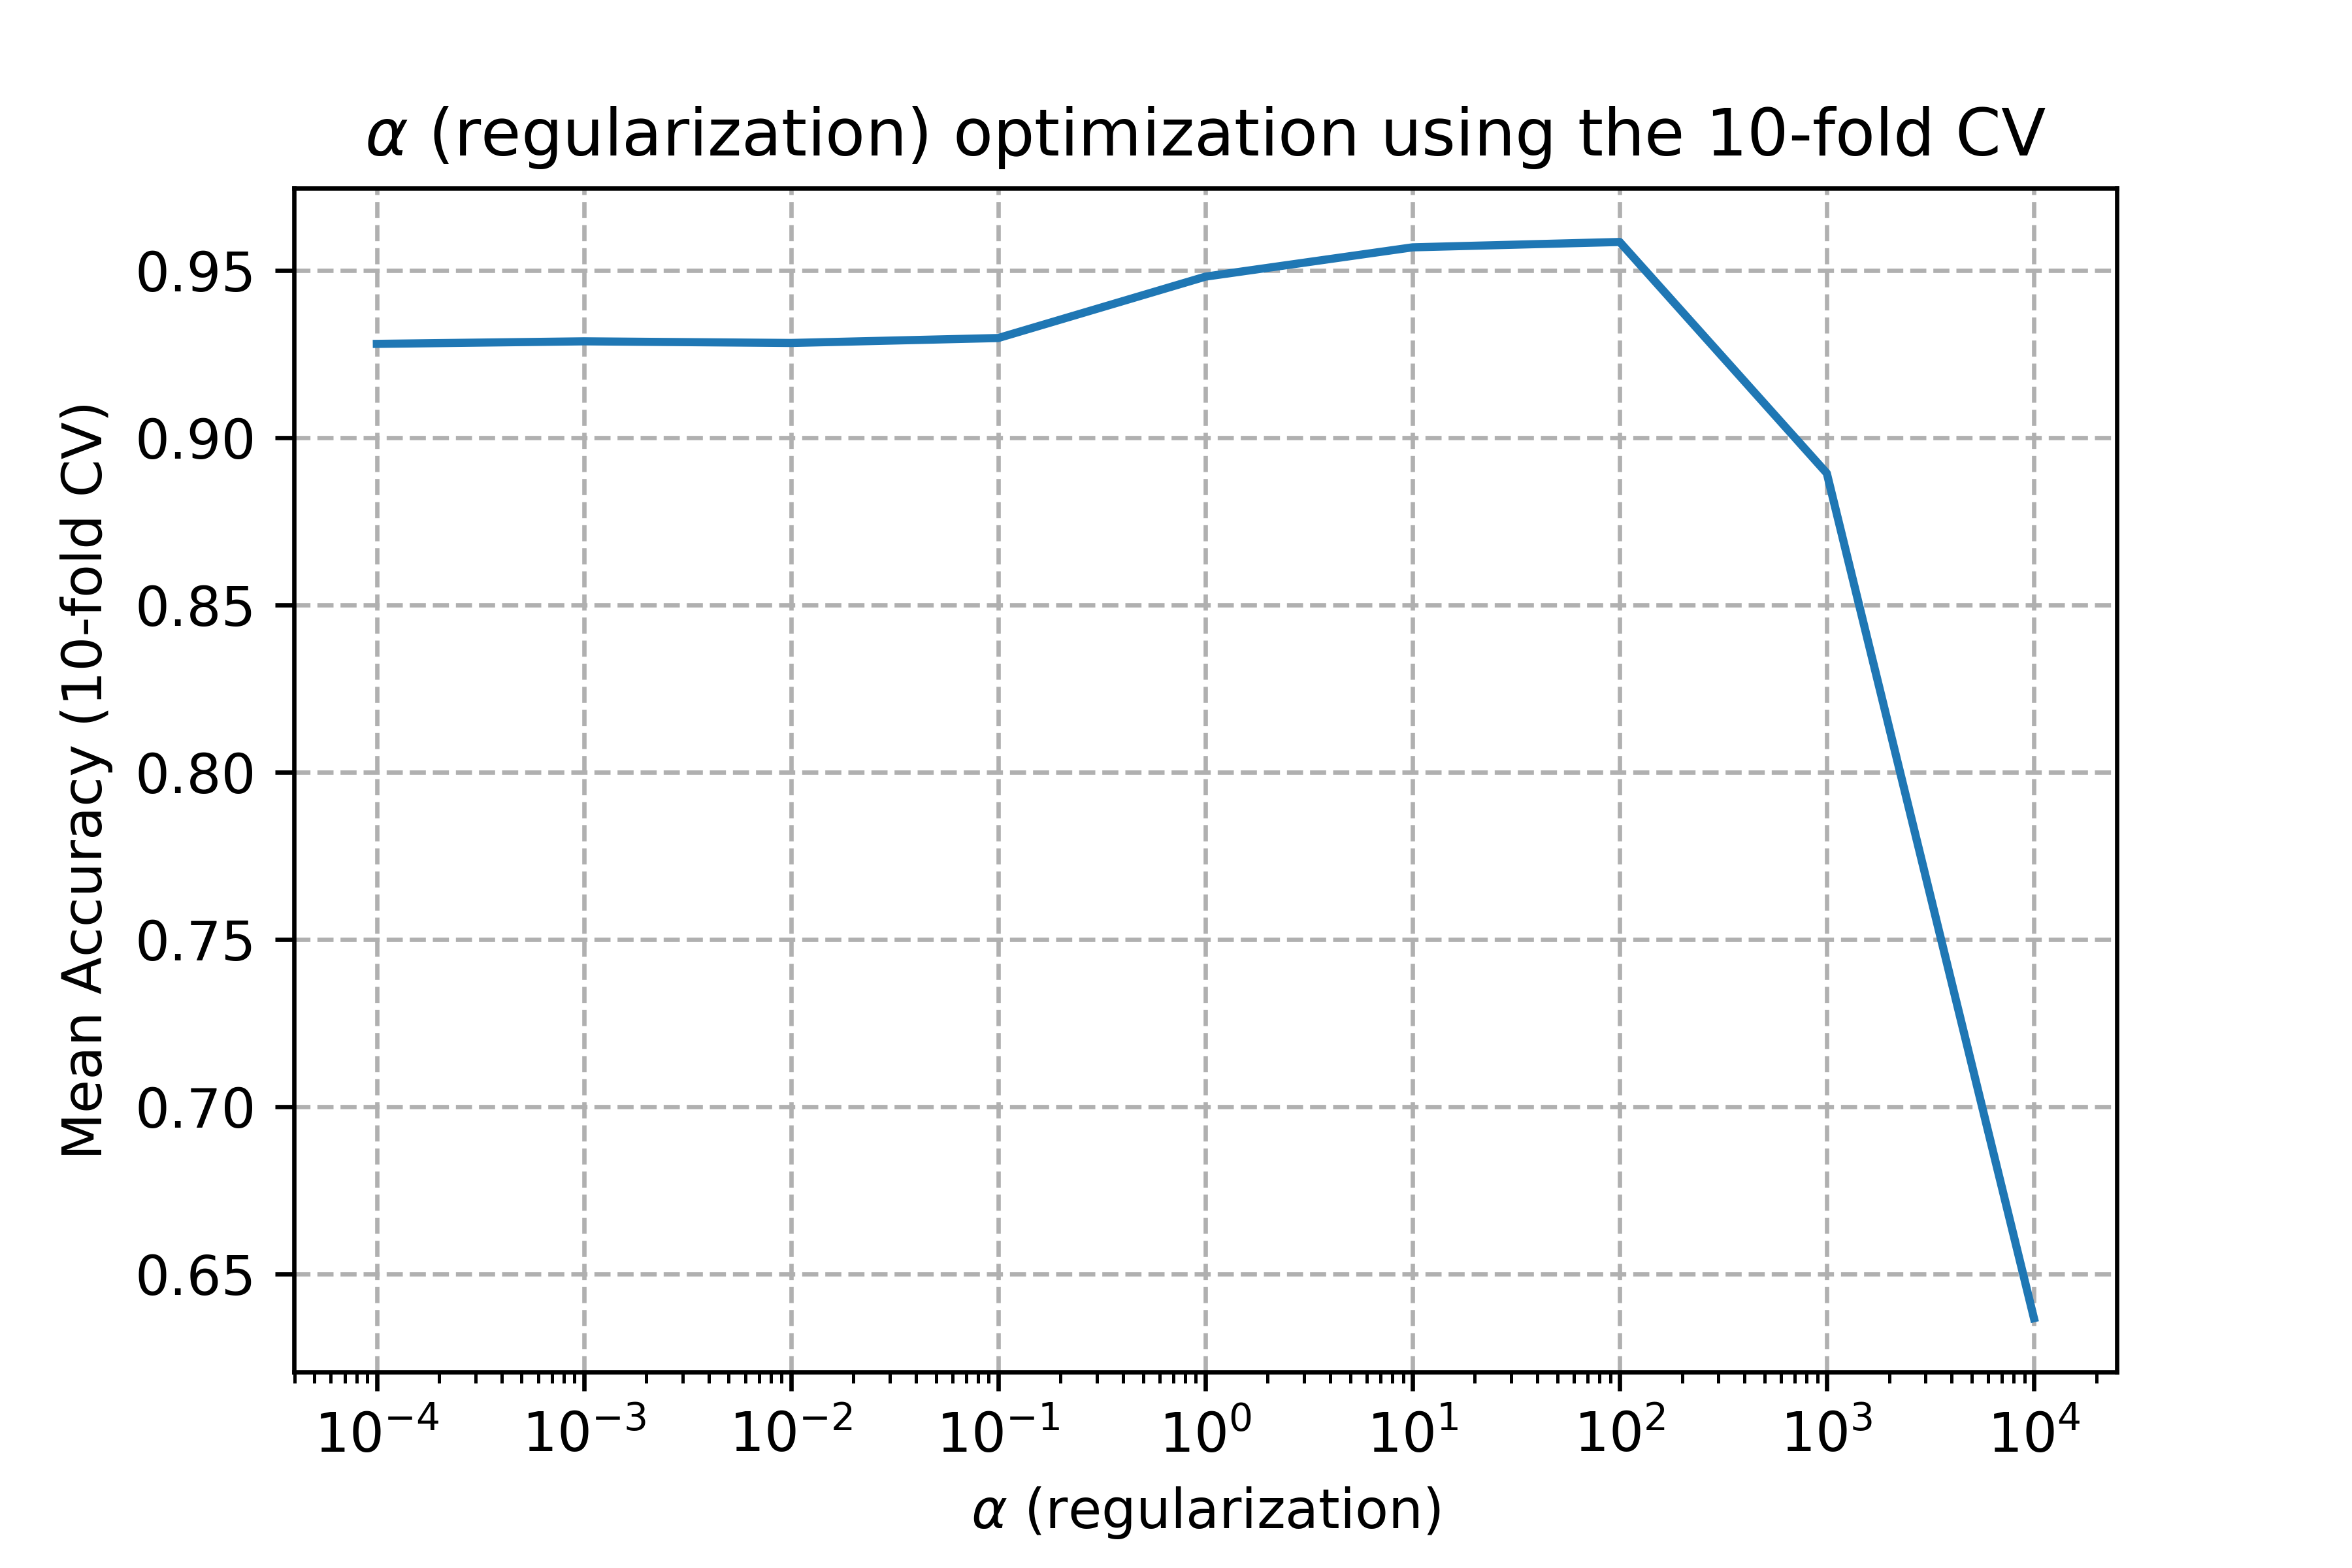
\includegraphics[width=0.33\linewidth]{figures/Neural_net_alpha_mean_acc.png}
\caption{CV for Neural networks. \label{fig:nn_cv}}
\end{figure}

\paragraph{Effect of number of samples on accuracy.}
For this experiment,  we progressively varied the fraction of samples used for training from 1\% to 100\% out of the entire 60,000 samples using randomized stratified sampling, taking the fraction of data from each class (digits 0-9) and combining them to form the training data and computed the accuracy on the test data (fixed size 10,000) for each case. Here we fixed the hyper-parameters for respective algorithm found using CV. The results are shown in Figure \ref{fig:svm_knn_accuracy_tss}.

From the plots we see that, approximately 20\% (12,000) of the training data points (60,000) is required for high accuracy. After 20\% data points, the accuracy 
almost remains in the same range even if we increase the number of training data points.

\begin{figure}[H]
	\centering
	\begin{subfigure}{0.4\linewidth}
		\centering
		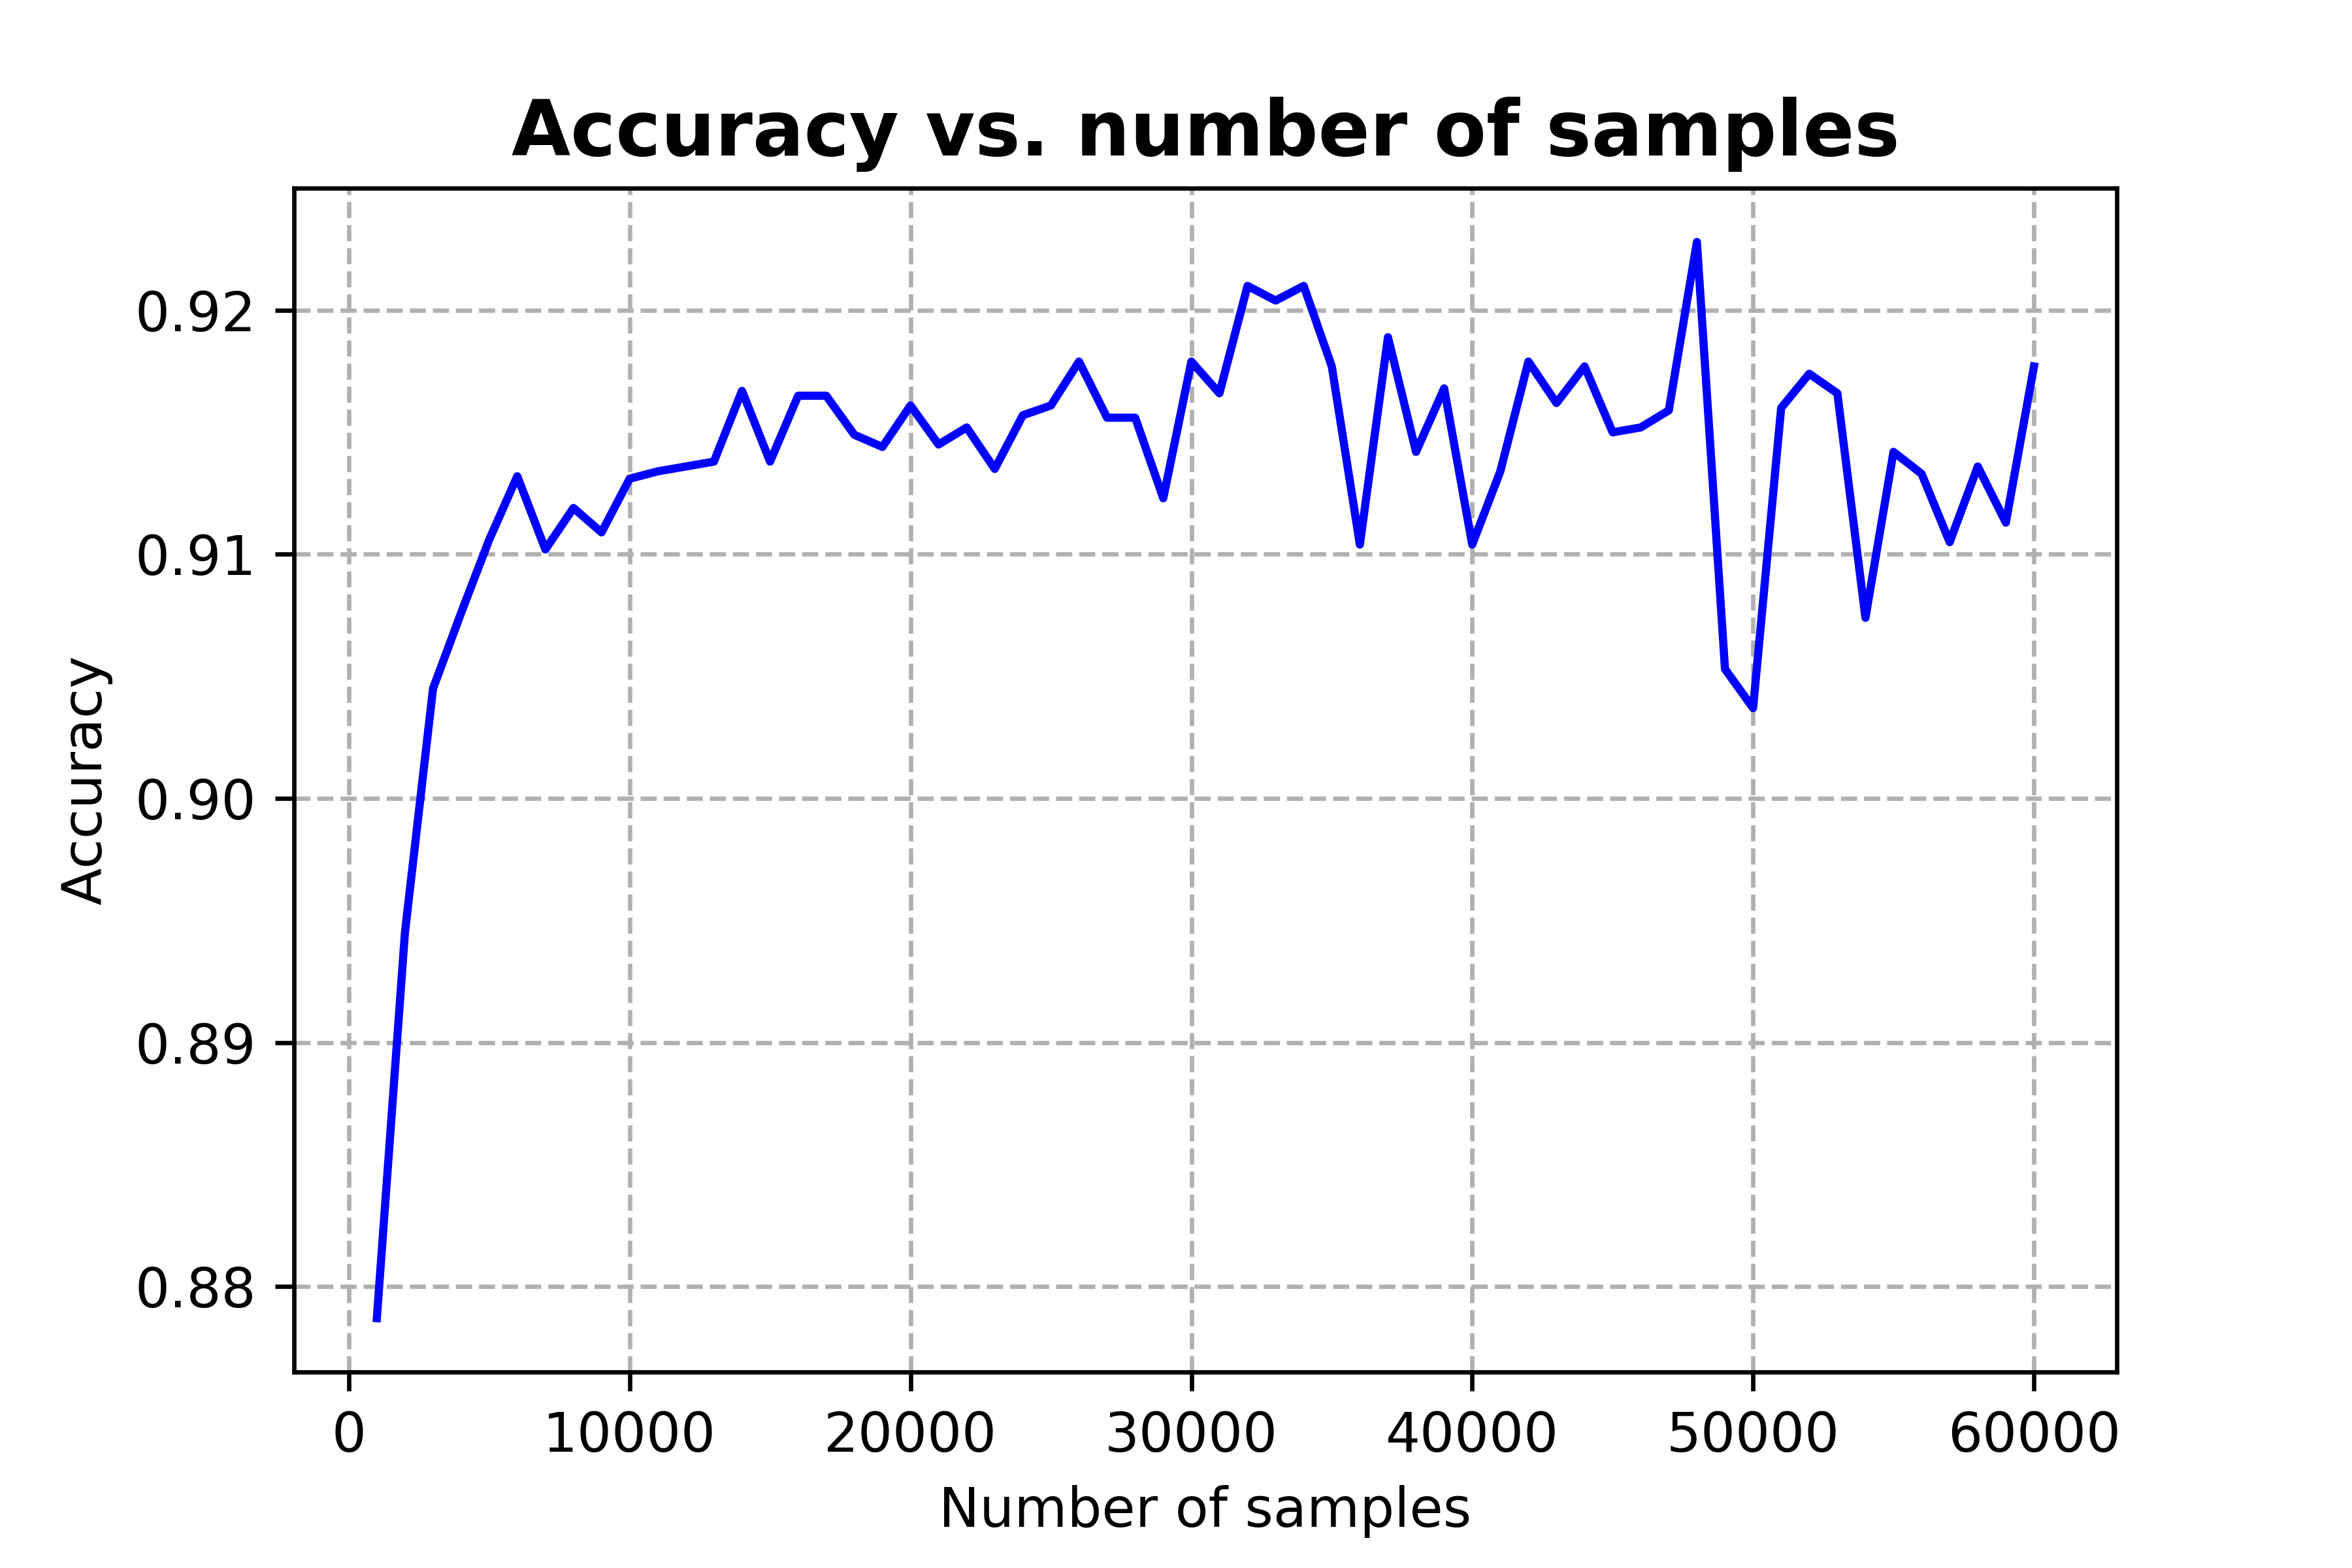
\includegraphics[width=1\linewidth]{figures/accuracy_vs_samples_linearsvm_default.png}
		\caption{SVM}\label{fig:1a}		
	\end{subfigure}
	\begin{subfigure}{0.35\linewidth}
		\centering
		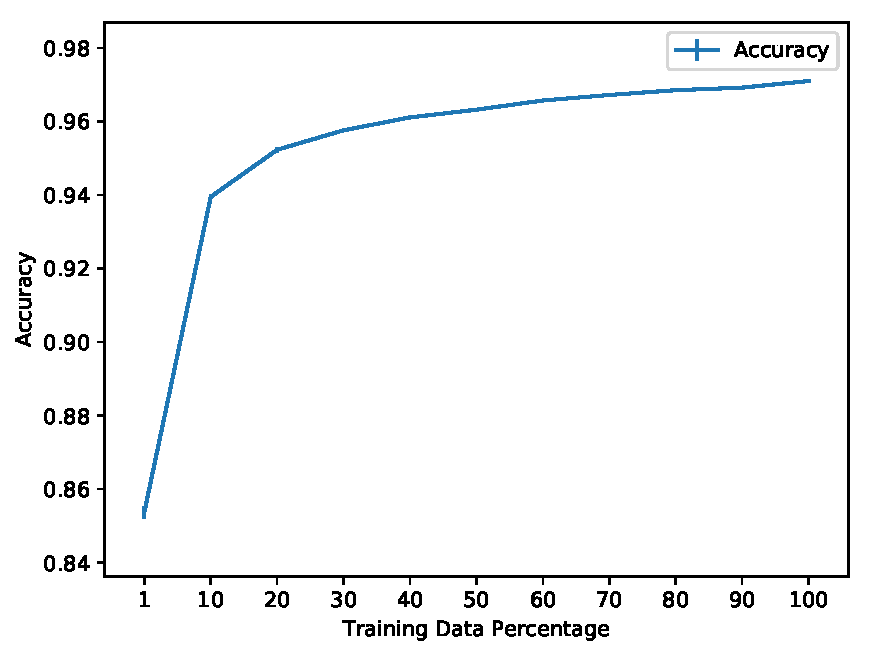
\includegraphics[width=1\linewidth]{figures/KNN_accuracy_vs_tss_with_fixed_k.pdf}
		\caption{KNN}\label{fig:1b}
	\end{subfigure}
	\begin{subfigure}{0.4\linewidth}
		\centering
		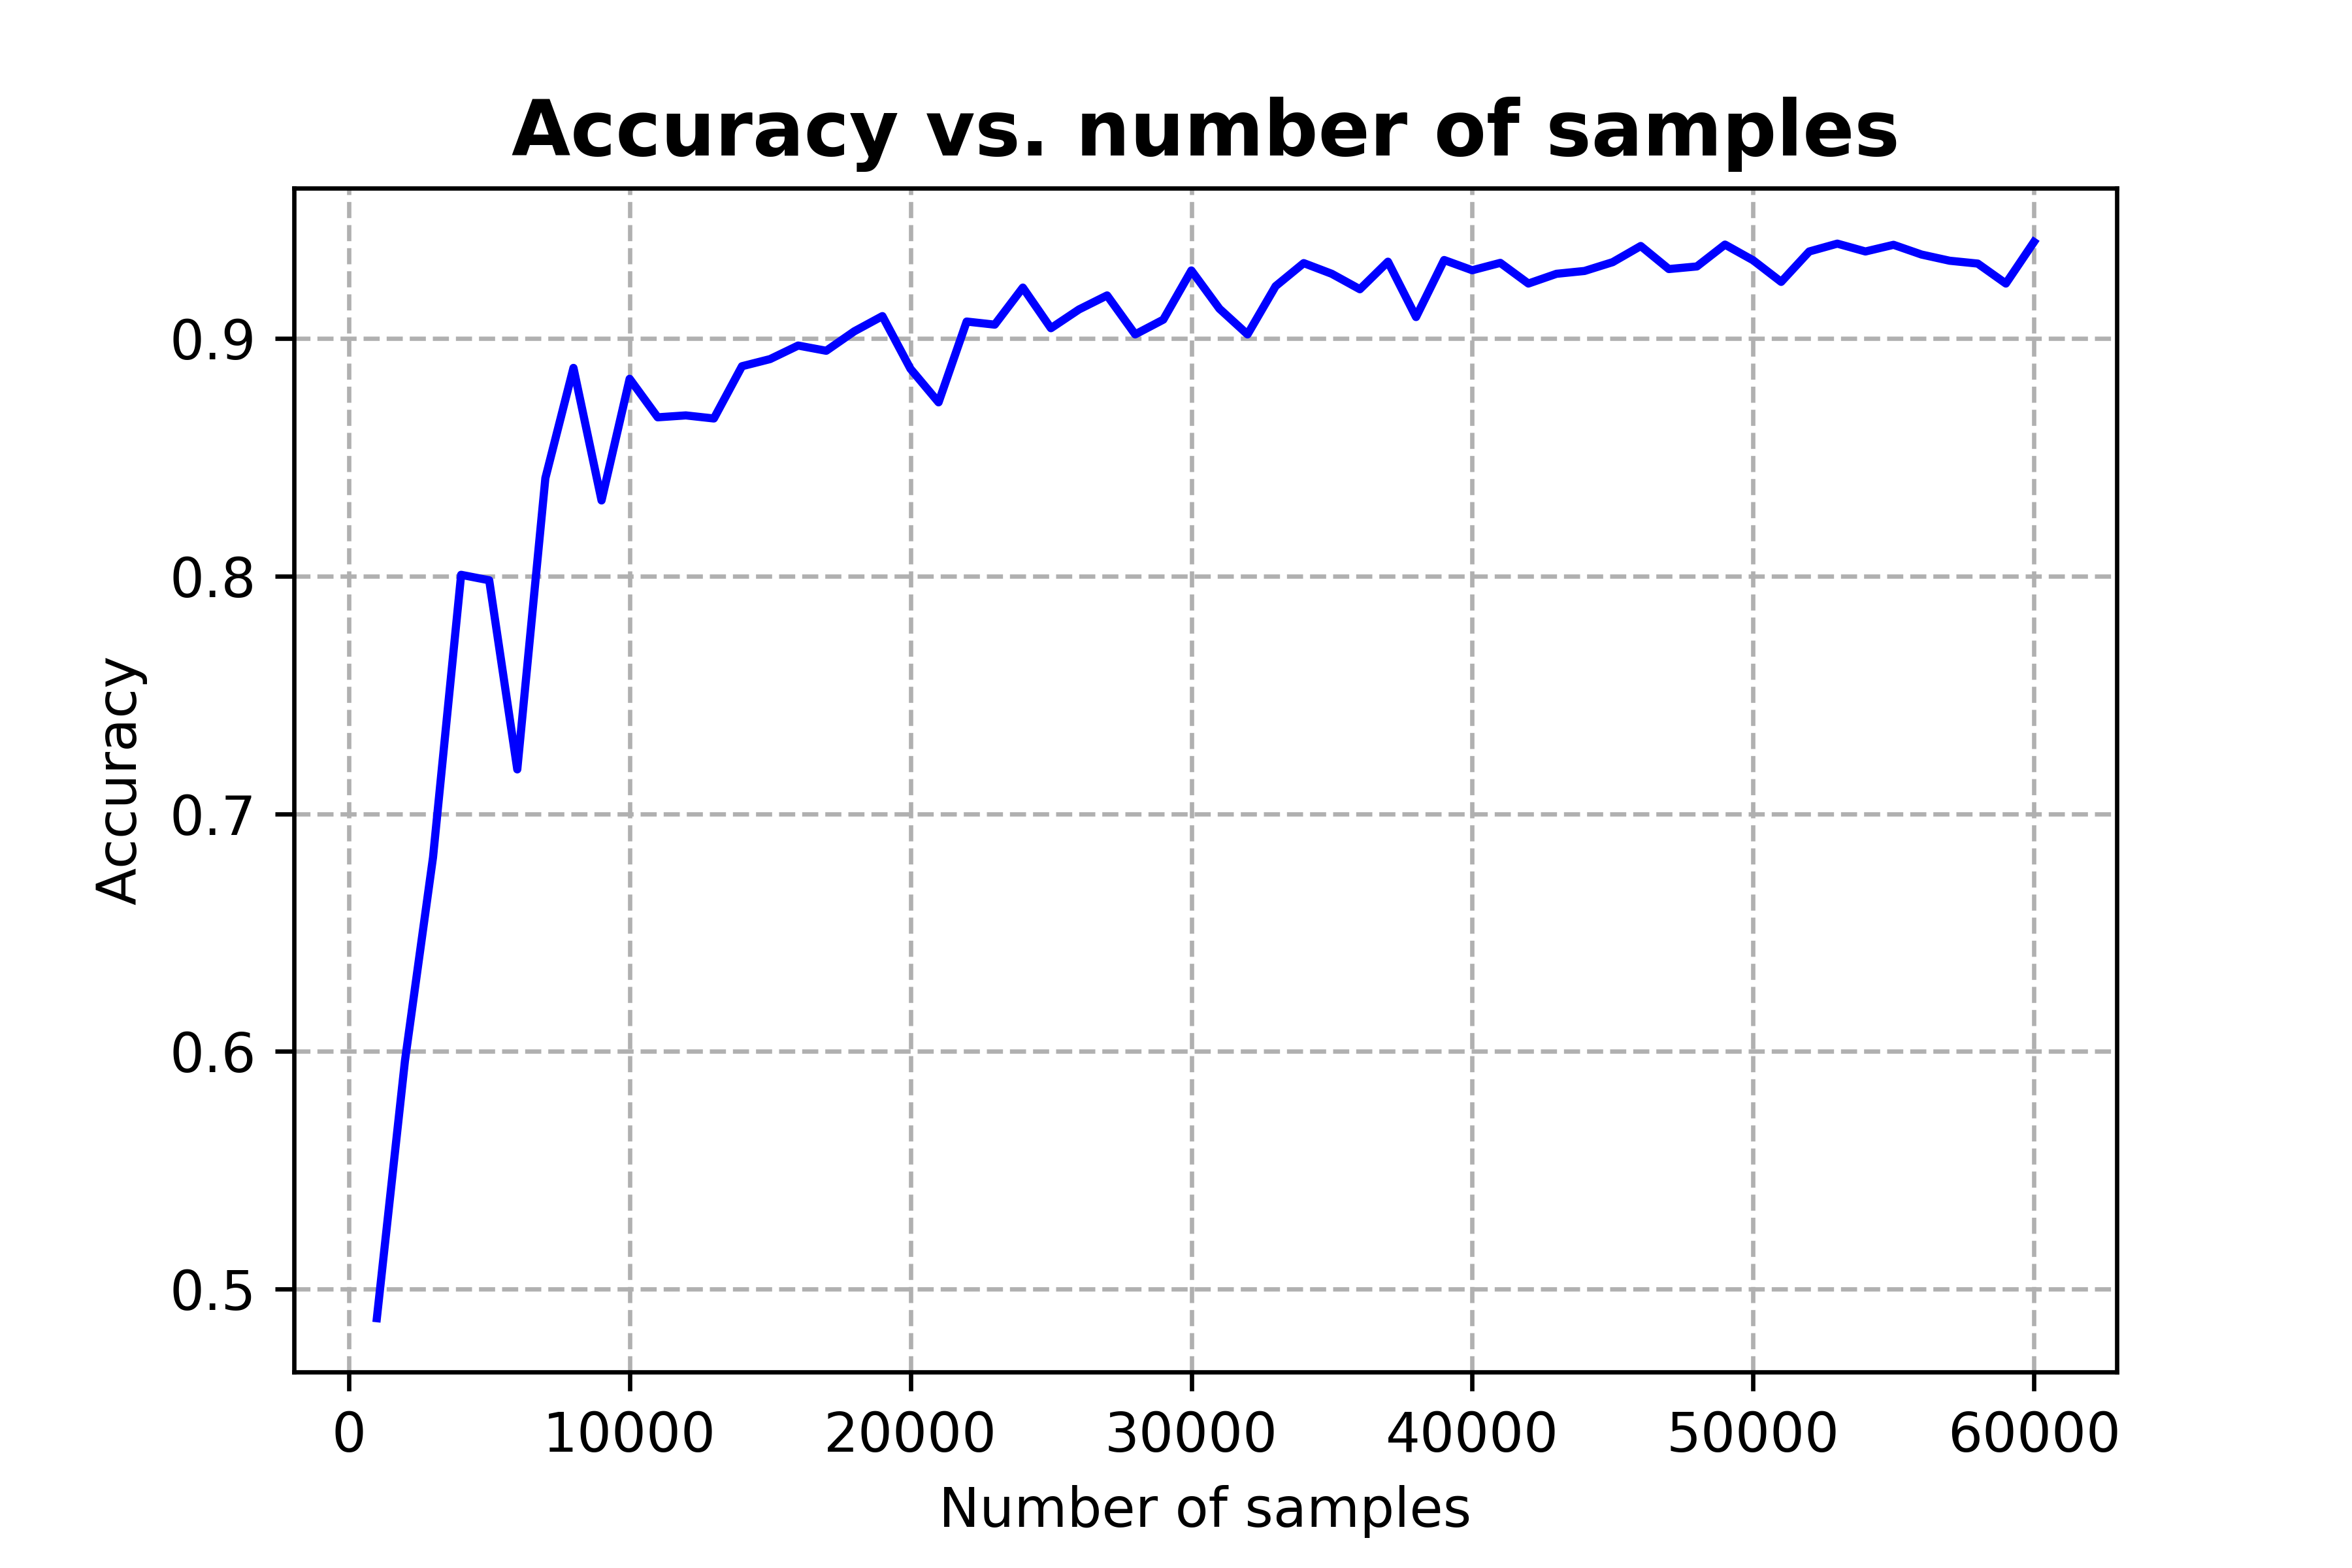
\includegraphics[width=1\linewidth]{figures/accuracy_vs_samples_neural_net_default}
		\caption{Neural Network}\label{fig:1b}
	\end{subfigure}
	\caption{Training set size vs. accuracy}\label{fig:1}
\end{figure}

\paragraph{PCA features.}
For this experiment, we computed the top-K principal component features such that the top-K principal components explained 90\% of the variance in the data. 
The results is shown in Figure \ref{fig:pca_features}.

From the plot we can see that the number PCA features are 87 out of 784 features which explains 90\% variance in the data.
\begin{figure}[H]
\centering
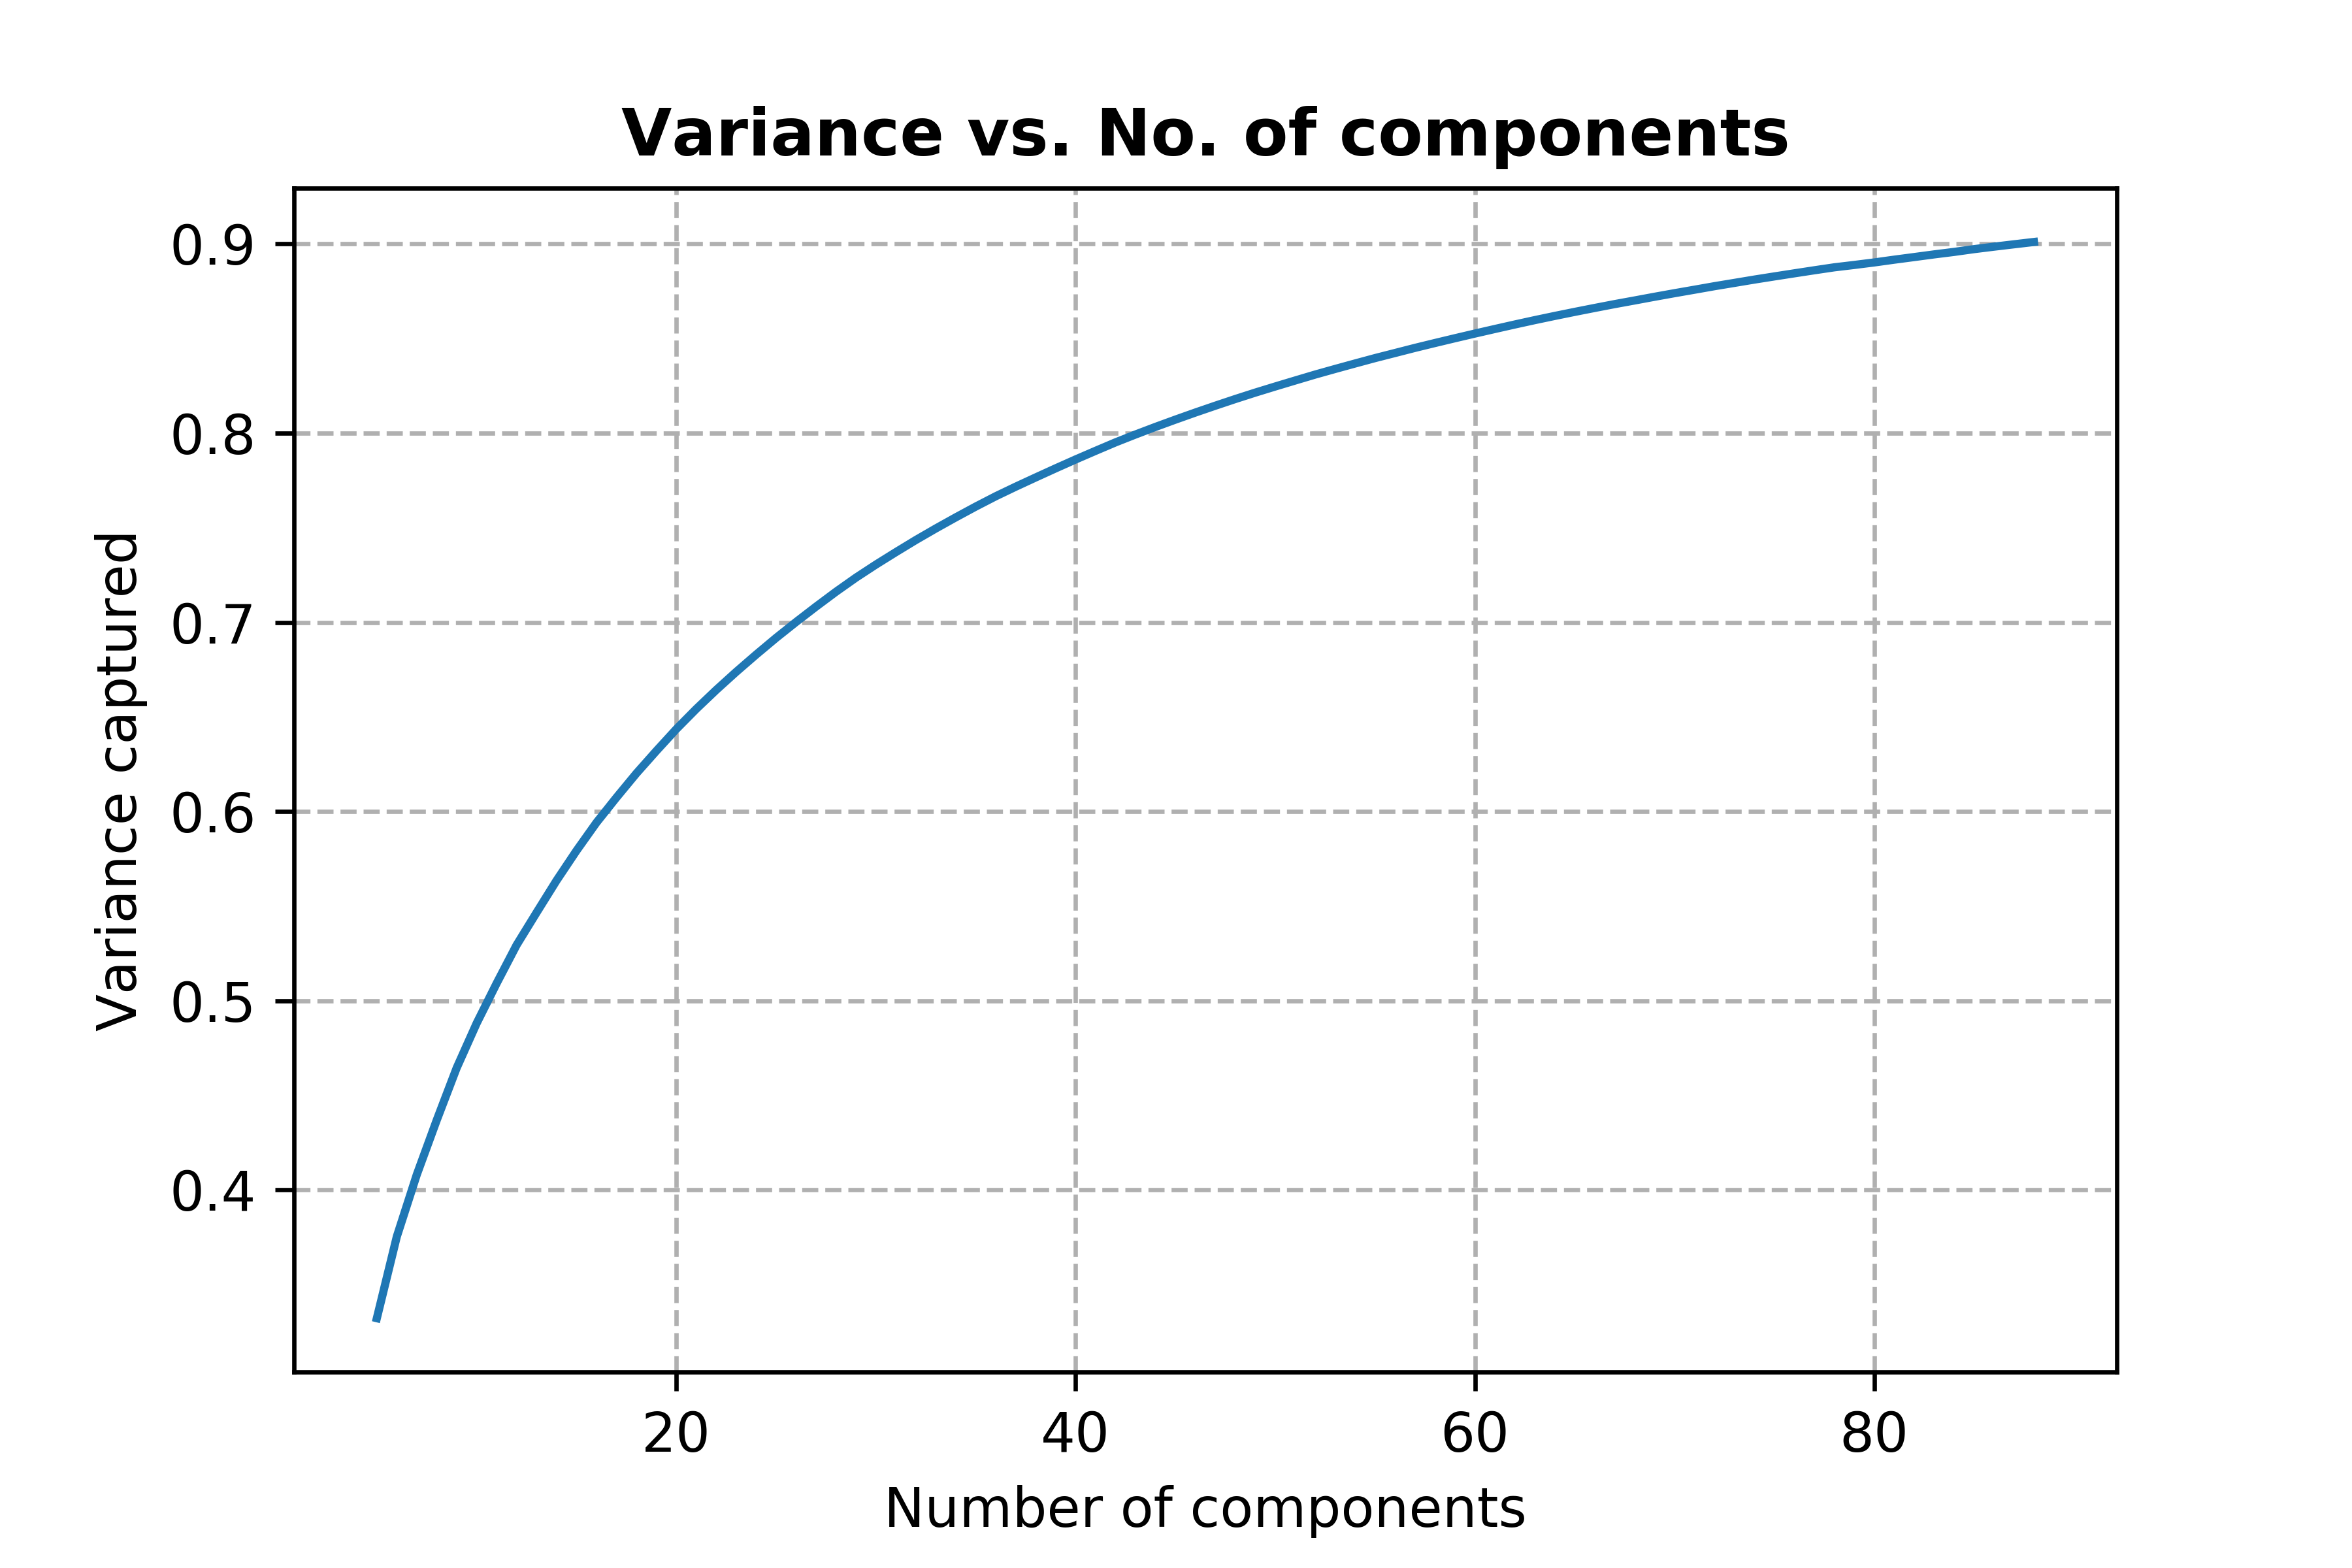
\includegraphics[width=0.5\linewidth]{figures/pca_variance_vs_no_comp.png}
\caption{PCA features. \label{fig:pca_features}}
\end{figure}
\section*{Work In-progress}
\begin{itemize}
\item We will generate some of the plots again with proper error bars. 
\item We would run several experiments to plot ROC curves for different algorithms.
\item We would run few experiments for all algorithms on the PCA features. 
\item Finally we would  run 10-fold cross validation for all the algorithms to do hypothesis testing to compare different algorithms.
\item We will include representative ROC curves for the 10-fold cross validation used for parameter tuning and for the test data-set that we would use for the hypothesis testing for choosing the best algorithm.
\item We will try to run more experiments for SVM (using RBF kernels) and generate results (This is tentative and we might not be able to finish it).
\item We will include data about run-times for different algorithms / parameter settings and discuss how that might be a deciding factor in selecting the parameters for different algorithms.
\end{itemize} 
\end{document}


